\documentclass[12pt]{article}
\usepackage[a4paper]{geometry}
\pdfoutput=1
% \usepackage{preiclr,times}
\usepackage{iclr2017_conference,times}
\usepackage[english]{babel}
\usepackage{hyperref}
\usepackage{url}
\usepackage{amssymb}
\usepackage{amsfonts}
\usepackage{amsmath}
\usepackage{graphicx}
\graphicspath{{images/}}
\usepackage{cleveref}
\usepackage{ccicons}
\usepackage{xcolor}
\definecolor{red-secondary-dark}{RGB}{205,32,38}
\usepackage{caption}
\usepackage[font={color=red-secondary-dark,small},figurename=Fig.,labelfont={it}]{caption}
\captionsetup[figure]{skip=0pt}
\usepackage[rightcaption]{sidecap}
\usepackage{floatrow}
\usepackage{framed}
\usepackage{mdframed}
\usepackage{lmodern}
\usepackage[most]{tcolorbox}
\newtcolorbox[blend into=figures]{blockfigure}[2][]{colback=white,
	float=!htbp,
	boxsep=0.5pt,left=2pt,right=2pt,top=0.5pt,bottom=0.5pt,
	center title,
	title={#2}, every float=\centering, #1}
\newtcolorbox[blend into=figures]{inlinefigure}[2][]{colback=white,
	boxsep=0.5pt,left=2pt,right=2pt,top=0.5pt,bottom=0.5pt,
	center title,
	title={#2}, every float=\centering, #1}
\usepackage[default]{sourcesanspro}
\usepackage[T1]{fontenc}
\usepackage{setspace}

\newtheorem{theorem}{Theorem}
\newtheorem{lemma}{Lemma}
\crefname{lemma}{Lemma}{Lemmas}
\newcommand\tab[1][1cm]{\hspace*{#1}}


\iclrfinalcopy


\begin{document}
\begin{titlepage}
	\begin{center}
		
\includegraphics[width=0.6\textwidth]{UnivAQ-logo}\\[1cm]
		{\large University of L'Aquila}\\[0.5cm]
		{\large Department of Information Engineering, Computer Science and Mathematics}\\[0.5cm]
		\rule{\linewidth}{0.5mm} \\[0.4cm]
		{\huge \bfseries Hyper Heursitic Cryptography\\
			with\\
			Mixed Adversarial Nets \\[0.4cm] }
		\rule{\linewidth}{0.5mm} \\[1.5cm]
		\noindent
		\begin{minipage}{0.4\textwidth}
			\begin{flushleft}
				\large
				\emph{Author :}\\
				Aly \textsc{Shmahell}
			\end{flushleft}
		\end{minipage}%
		\begin{minipage}{0.4\textwidth}
			\begin{flushleft}
				\large
				\emph{Supervisor :} \\
				Prof.~Giovanni \textsc{De Gasperis}\\
			\end{flushleft}
		\end{minipage}
		\vfill
		\today
	\end{center}
\end{titlepage}
\begin{titlepage}
		\begin{center}
			
\includegraphics[angle=-90]{by-nc-sa}
		\end{center}
			\begin{center}
				This dissertation is licensed under a
			\end{center}
			\begin{center}
				 \href{http://creativecommons.org/licenses/by-nc-sa/4.0/}{Creative Commons Attribution-NonCommercial-ShareAlike 4.0 International License.}
			\end{center}
		
\end{titlepage}
\begin{abstract}
Abstract
\end{abstract}
\newpage
\section{\textbf{Introduction}}\label{sec:introduction}
Neural cryptography is an interdisciplinary field in Computer Science, combining both Artificial Intelligence and Cryptography, towards the development of stochastic methods, based on artificial neural networks, for use in encryption and cryptanalysis.
\subsection{\textbf{Paper Objective}}
The objective of this paper is to explore the use of new developments in the field of Neural Networks, mainly Adversarial Neural Networks and Convolutional Neural Networks, as a generative model, to produce a new breed of Crypto-Systems.\\\\
The work being done here is based on a new paper released in 2016 from Google's DeepMind, which promises to bridge the gap between research and application in this area.\\\\
The goal of my research is to provide the following:
\begin{itemize}
	\item an addition to the variety of methods provided in the original paper.
	\item an improvement in performance of the models being built.
	\item an in-depth analysis of how the components work, and the inner details of their mechanics.
	\item a software documentation that provides a blueprint for a more software-engineering oriented neural-cryptosystem prototype.
\end{itemize}
With the research paper specter in this area being dominated by authors coming from a mathematical-background angle, my paper aims to provide:
\begin{itemize}
	\item a Computer Science oriented approach to solving cryptography with neural networks and stochastic methods.
\end{itemize}
This paper finally adds the following:
\begin{itemize}
	\item the introduction of hybrid neural crypto-systems.
	\item an exploration into adding hyper heuristics to the field.
\end{itemize}
\newpage
\subsection{\textbf{Paper Motivation}}
The question of motivation can be empirically divided into:
\begin{itemize}
	\item Why is the idea of importance?
	\item Why does the author think it would work?
\end{itemize}
\textbf{Why is Neural Cryptography of importance?}\\
The age of intelligent machines is comprised of multiple intricate components, but individually they function narrowly even for the simplest of tasks, but the surge of incorporation of these multiple components into the backbone of neural-nets has put artificial intelligence on a fast track towards competence in multiple complex areas of problem solving, surpassing human intelligence by multitudes on many occasions.\\\\
It makes sense from an academic perspective that we want neural nets to incorporate an understanding of cryptography.\\
It also makes sense from an economic and existential point that we want these backbones of machine intelligence to parallel their success in surpassing human intelligence on cryptography, in order to open the door for new opportunities in that area.\\\\
\textbf{Why would Neural Cryptography work?}\\
This boils down to multiple general factors:
\begin{itemize}
	\item The incorporation of multiple heuristic methodologies into one unified backbone, which made it tackle a rapidly growing heap of complex tasks, cryptography is just another human invention to be caught up with.
	\item The increasing successful research into using these heuristics not just to compute a complex task, but to do it quickly without loss in accuracy.
	\item The introduction of tools, frameworks and libraries of industrial level to the public which propelled the field of neural networks and made it ever so easy to replicate experiments and improve upon them.
\end{itemize}
Which lead to those paper-related factors:
\begin{itemize}
	\item The introduction of Convolutional networks provides a well tested and understood methodology in reducing problems where local spatial relations in the data matter, which is the case for cryptography and cryptanalysis.
	\item Having a Mixed Convolutional Net with a fully connected layer will teach the network to account for global spatial relations as well.
	\item A result of using Convolutions is that the small-sized pattern-finding filter has shared weights (and biases) for all spatial locations which the convolution processes, which reduces the compute-power required for the whole process compared to other network models.
	\item Adversarial computation has been proven to be effective for years in the form of Genetic Algorithms, and adding adversary as a non-supervised generative model provides a better and easier experiment on how to synthesize a new form of cryptography.
\end{itemize}
\newpage
\subsection{\textbf{Xavier Initialization} \cite{DBLP:journals/jmlr/GlorotB10}}
When we talk about initialization, we mean the initial value which should be given to a certain neuron, this initial value is important for the neuron and for the network in general.\\
\begin{lemma}\label{lemma1}
Suppose our net uses the hyperbolic tangent activation function for its neurons:\\
\begin{blockfigure}{example plot of the hyperbolic tangent}
	\[ 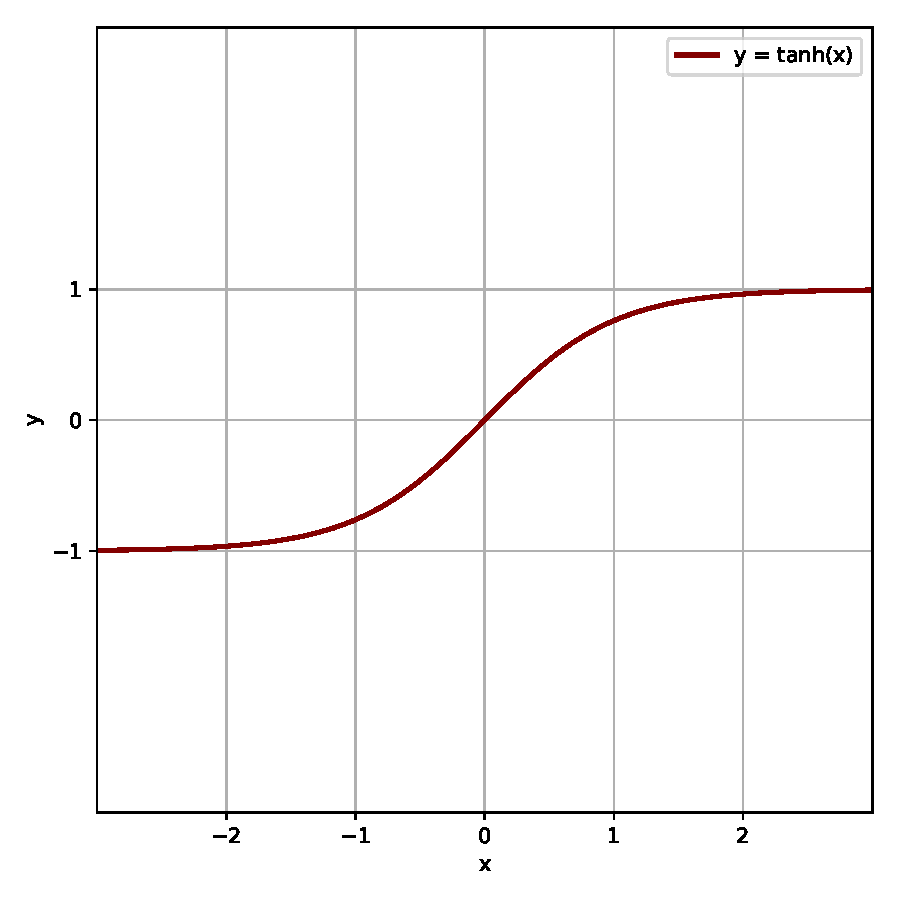
\includegraphics[width=0.6\textwidth]{tanh} \]
\end{blockfigure}
\begin{itemize}
	\item If the weights start too small, then the signal shrinks as it passes through each layer until it vanishes, then as it passes deeper in the network with its small values, the layers it enter will become linear, because the output of the hyperbolic tangent is linear with small input values, this means the deeper layers of the net will loose non-linearity.
	\item If the weights start too large, then the signal grows as it passes through each layer until it becomes too large, then as it passes deeper in the network with its large values, the layers it enter will become saturated, as the output of the hyperbolic tangent is flat with large input values, and this flatness will cause the gradient to become zero, and we will get the vanishing gradient problem.
\end{itemize}
\end{lemma}
\begin{lemma}\label{lemma2}
Having a pre-defined net graph: for each neuron we know the number of inputs and the number of outputs, therefor we can calculate a reasonable weight for the neuron in question based on a normal distribution of a zero mean and a 1/n variance.
\end{lemma}
\begin{lemma}\label{lemma3}
To achieve initialization while avoiding the two obstacles in \cref{lemma1}, we want the variance to remain the same with each passing layer.	
\end{lemma}
\newpage
Suppose we have an input X from a previous layer with n components and a linear neuron with random weights W in the current layer that spits out the same output Y to some neurons in the next layer.
\begin{blockfigure}{Xavier Initialization on neuron "n"}
		\[ 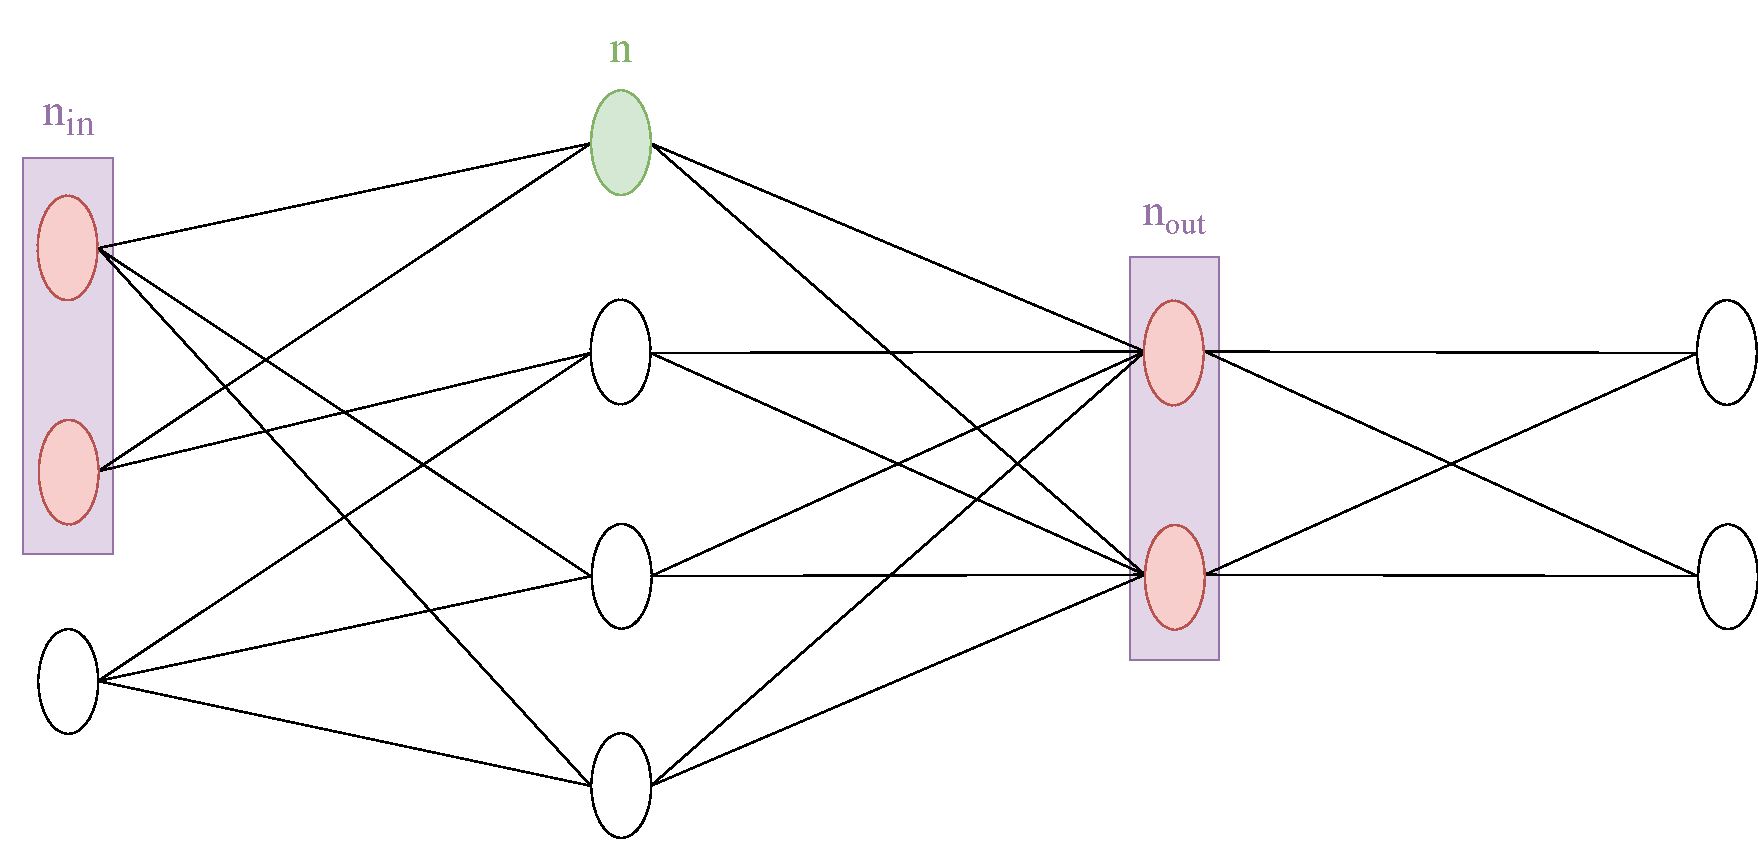
\includegraphics[width=0.6\textwidth]{xavier_illustration} \]
\end{blockfigure}
The output of the neuron will have the following equation:
\begin{center}
	\begin{equation}
		Y = W_1X_1 + W_2X_2 + ... + W_n X_n \label{eq:1}
	\end{equation}
\end{center}
To calculate the variance of each component:
\begin{center}
	\begin{equation}
		Var(W_iX_i) = E[X_i]^2 Var(W_i) + E[W_i]^2 Var(X_i) + Var(W_i)Var(X_i) \label{eq:2}
	\end{equation}
\end{center}
Since our inputs and weights come from a normal distribution of zero mean (from \cref{lemma2}):
\begin{center}
	\begin{equation}
		E[X_i]^2 Var(W_i) + E[W_i]^2 Var(X_i) = 0 \implies
		Var(W_iX_i) = Var(W_i)Var(X_i) \label{eq:3}
	\end{equation}
\end{center}
Since the neurons in the same previous layer are all independent, we assume that both $ X_i $ and $ W_i $  are independent and also identically distributed:
\begin{center}
	\begin{equation}
	 Var(Y) = Var(W_1X_1 + W_2X_2 + ... + W_n X_n) = nVar(W_i)Var(X_i) \label{eq:4}
	\end{equation}
\end{center}
In the last equation, we have the variance of the inputs, the variance of the output and the variance of the weights, now we can calculate the variance of the weights from ~\cref{lemma3}:
\begin{center}
	\begin{equation}
	 Var(Y) = Var(X_i) \implies Var(W_i) = \frac{1}{n_{in}} \implies Var(W_i) * n_{in} = 1  \label{eq:5}
	\end{equation}
\end{center}
Now if we go through the same derivation for back-propagation, we get:
\begin{center}
	\begin{equation}
	Var(W_i) = \frac{1}{n_{out}} \implies Var(W_i) * n_{out} = 1 \label{eq:6}
	\end{equation}
\end{center}
To keep the variance of the input gradient \& the output gradient the same, we combine
\eqref{eq:5} \& \eqref{eq:6} and we get:
\begin{center}
	\begin{equation}
	(n_{out} + n_{in}) * Var(W_i) = 2 \implies Var(W_i) = \frac{2}{n_{in} + n_{out}} \label{eq:7}
	\end{equation}
\end{center}
\newpage
\subsection{\textbf{1D Convolution on Batch 1D Data with (1,2)-D Filters}}
1D Convolution works by sliding along 1 axis, then performing matrix multiplication, therefor in order to perform 1D convolution with a 2D filter, we need to add another axis to our data.\\\\
However, if our data is a batch of samples, then each sample has 1D convolution performed on it separately, that calls for adding another axis to both our data and our filter, in order to re-do the convolution on each data sample separately.\\\\
Therefor we end up with a 3D tensor for the batch data, and another 3D tensor for the filter.\\\\
To illustrate how this works, I've chosen a flat representation of the 3D tensors (representing 3D with 2D), mainly because this is how it's done with Numpy, and this is more practical for practitioners.\\\\
\begin{blockfigure}{Flat Axis Representation of 3D Tensors - Numpy Style}
		\[	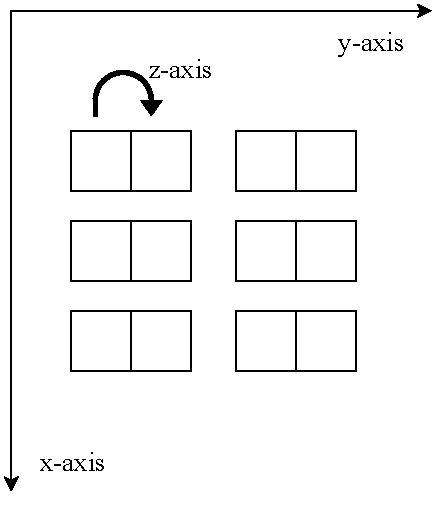
\includegraphics[height=0.3\textheight]{numpy-3Dtensor-axis} \]
\end{blockfigure}
1D Convolution slides over the y-axis for one convolution on a 1D sample, everything on the same index on the y-axis belongs to that one sample, and the multiplication is performed for that sample independent of the others.\\\\
On the other hand, 1D convolution considers the filter as a whole, and slides over the x-axis of the filter when convolving on one data sample.\\\\
The multiplication is done by multiplying the z-axis from the data sample by the y-axis from the filter, along the x-axis of the filter.\\\\
Then sliding is performed, and the multiplication is applied again.\\\\
when the filter cannot multiply anymore (out of reach), then convolution over this sample is over.\\\\
Once that happens, the filter is slided to its default position, then we slide over the x-axis to perform 1D convolution again on another data sample from the batch.
\newpage
The following is an example of 1D convolution over a batch of 1D data with a 2D filter:\\\\
\tab The example starts off by generating 1D input strings.\\
\begin{tcbraster}[raster columns=3,raster rows=3,
	enhanced,size=small,fit algorithm=hybrid* ]
	\begin{inlinefigure}{First Input String}
		\begin{center}
			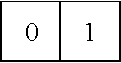
\includegraphics[width=0.5\textwidth]{input1}
		\end{center}
	\end{inlinefigure}
	\begin{inlinefigure}{Second Input String}
		\begin{center}
			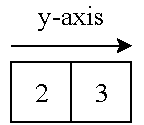
\includegraphics[width=0.5\textwidth]{input2}
		\end{center}
	\end{inlinefigure}
	\begin{inlinefigure}{Third Input String}
		\begin{center}
			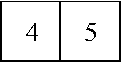
\includegraphics[width=0.5\textwidth]{input3}
		\end{center}
	\end{inlinefigure}
\end{tcbraster}
\tab Input strings are then stacked up along the x-axis to form a 2D batch.
\begin{blockfigure}{Input Batch}
	\begin{center}
		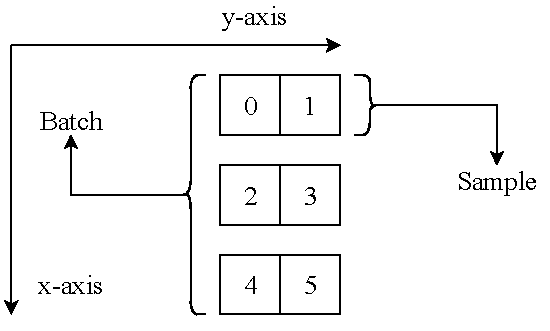
\includegraphics[width=0.4\textwidth]{input_final}
	\end{center}
\end{blockfigure}\\
\tab Then the batch gets expanded from 2D to 3D along the y-axis (injecting z-axis into y-axis), \tab which means the final batch shape becomes (3, 2, 1).
\begin{blockfigure}{Reshaped Input Batch}
	\begin{center}
		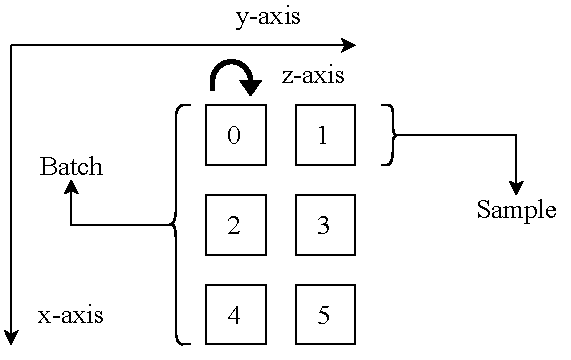
\includegraphics[width=0.4\textwidth]{input_reshaped}
	\end{center}
\end{blockfigure}\\
\tab Then finally, a filter of shape (2, 1, 2) is provided for the convolution.
\begin{blockfigure}{Filter \#1 with arbitrary weights}
	\begin{center}
		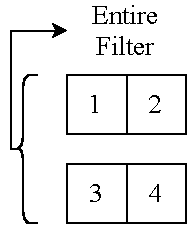
\includegraphics[width=0.17\textwidth]{filter1}
	\end{center}
\end{blockfigure}
\newpage
\begin{blockfigure}{ Applying the filter to the first sample in the input batch - generating the first value for the first  in the first feature map.}
	\begin{center}
		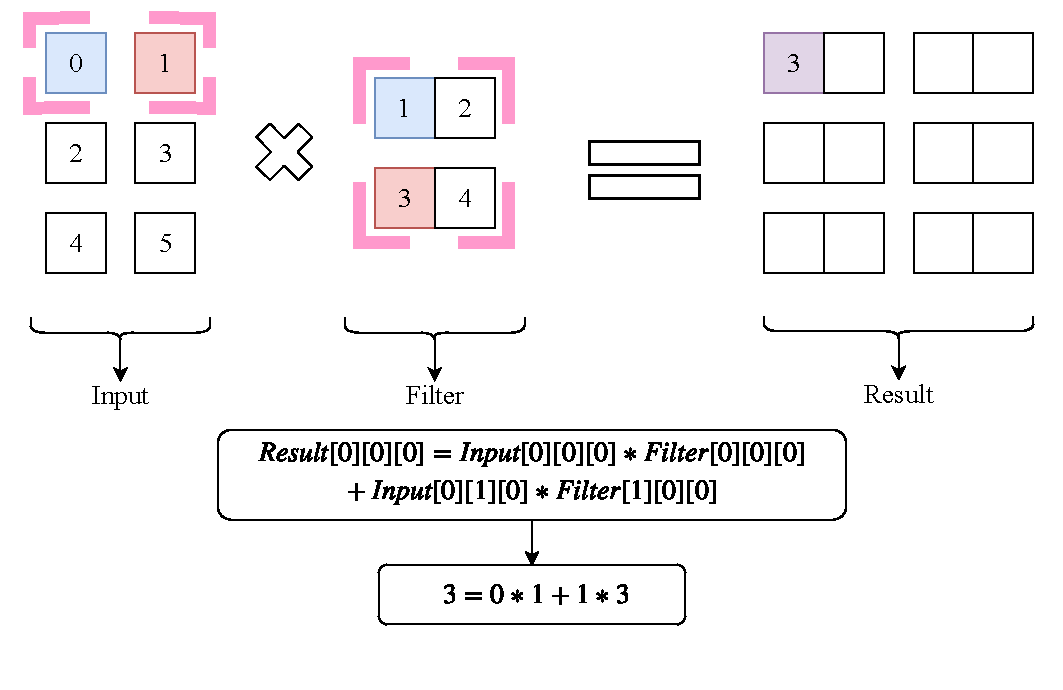
\includegraphics[width=\textwidth]{firstConvSample_step1}
	\end{center}
\end{blockfigure}
\begin{blockfigure}{ Applying the filter to the first sample in the input batch - generating the second value in the first feature map.}
	\begin{center}
		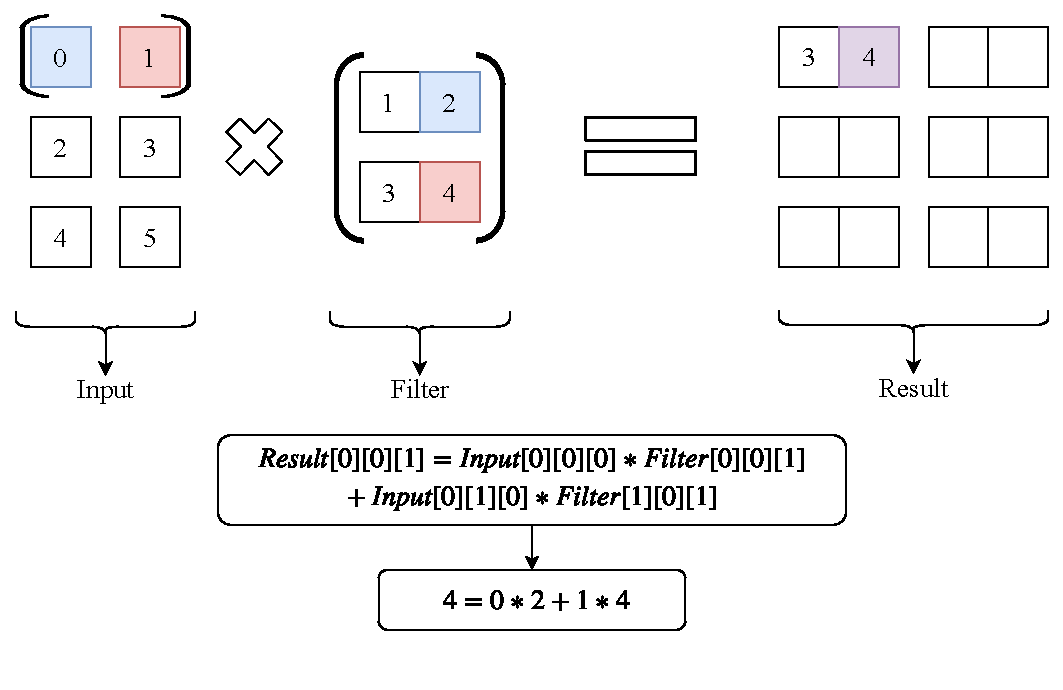
\includegraphics[width=\textwidth]{firstConvSample_step2}
	\end{center}
\end{blockfigure}
\newpage
\begin{blockfigure}{ Applying the filter to the first sample in the input batch - generating the second feature map.}
	\begin{center}
		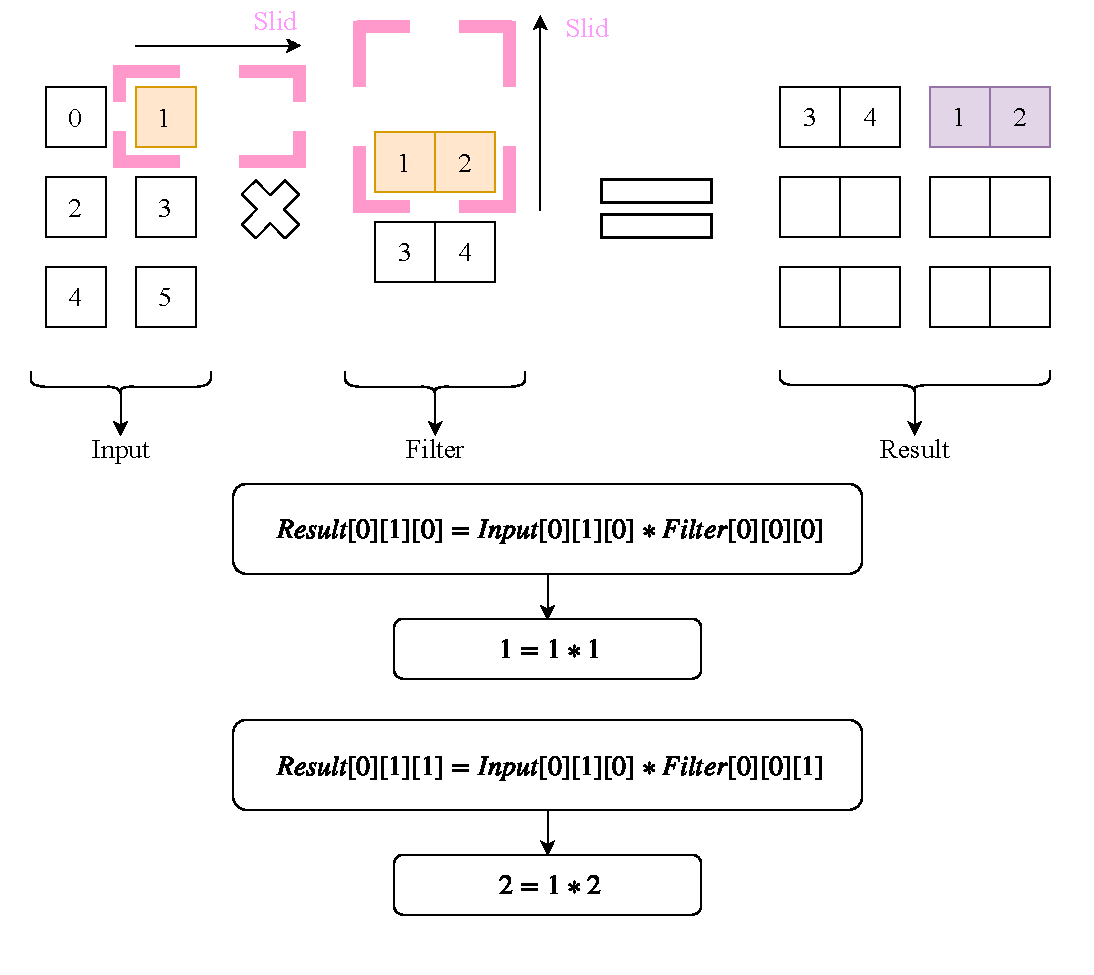
\includegraphics[width=\textwidth]{firstConvSample_step3}
	\end{center}
\end{blockfigure}
\begin{blockfigure}{ The entire convolution performed on the batch data.}
		\begin{center}
			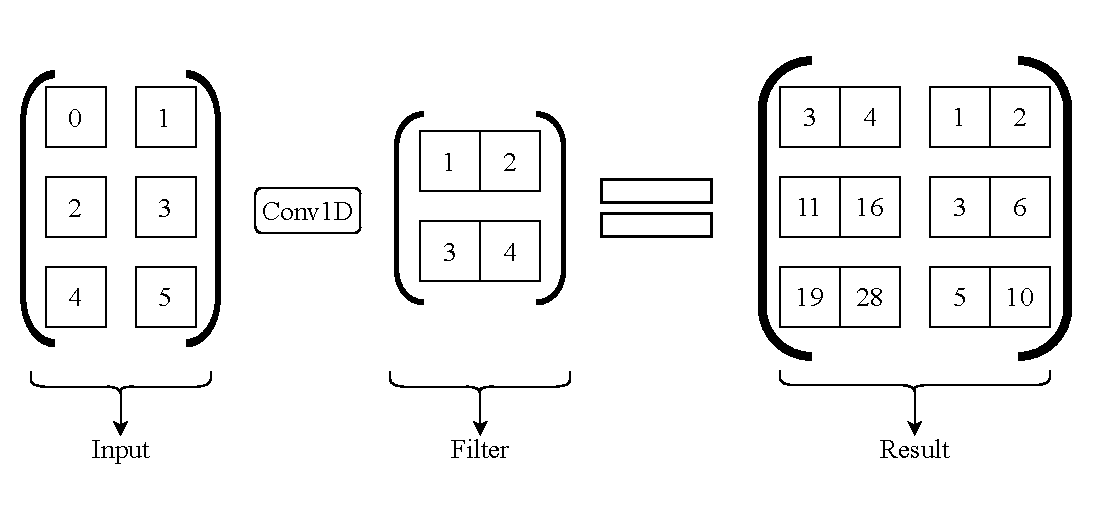
\includegraphics[width=\textwidth]{firstConvSample_final}
		\end{center}
\end{blockfigure}
\tab The resulting 3D tensor is of shape (3, 2, 2), and evident by its x-axis, it contains 2 feature \tab maps.
\newpage
To continue with the example, the resulting tensor from the previous convolution can be run through another convolution, for this purpose we need a new filter that conforms to the rules of matrix multiplication (taking into account the sliding rule), that is its y-axis has the same length as the z-axis from the tensor we're convolving on.\\\\
Also, the x-axis of the filter should be larger or equal to the y-axis of the tensor being convolved on.\\\\
And for the sake of making the example closer to real-life usage, we will make the resulting tensor from this new convolution have the same shape as the original input tensor by making the z-axis of the new filter of length 1, which will reduce the number of feature maps from 2 to 1, then by performing dimensionality reduction (squeezing of the z-axis onto the y-axis).\\\\
The shape of the newly constructed filter would be: (var, 2, 1), where $ var \>= 2 $, in our example var = 3.
\begin{blockfigure}{The output from the first conv layer becomes input to the second conv layer}
	\begin{center}
		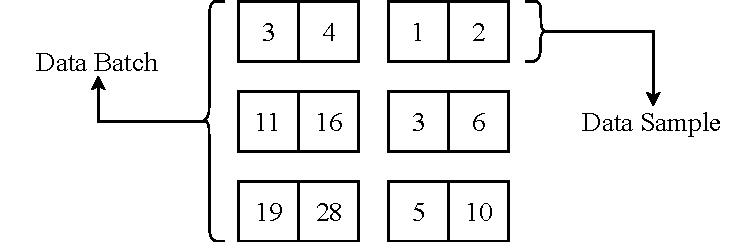
\includegraphics[width=\textwidth]{secondinput_final}
	\end{center}
\end{blockfigure}
\begin{blockfigure}{Filter \#2 with arbitrary weights}
	\begin{center}
		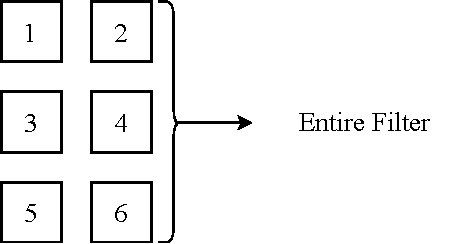
\includegraphics[width=\textwidth]{filter2}
	\end{center}
\end{blockfigure}
\newpage
\begin{blockfigure}{ Extracting the first value from the first sample in the data tensor to the feature map.}
	\begin{center}
		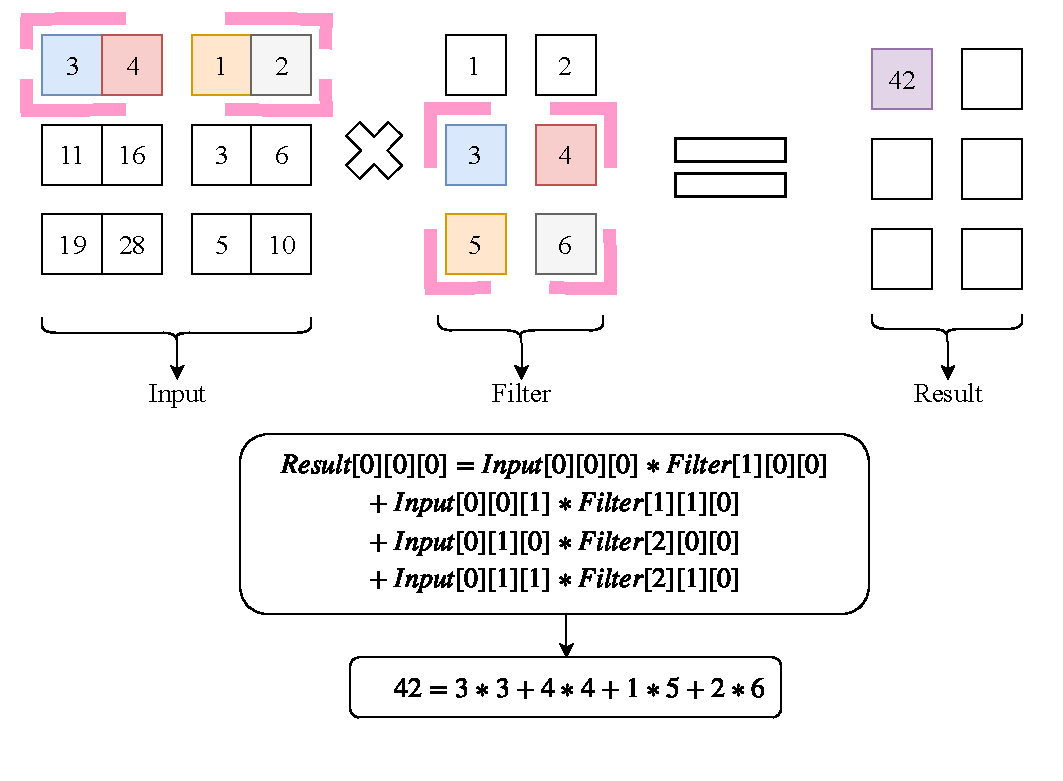
\includegraphics[width=\textwidth]{secondConvSample_step1}
	\end{center}
\end{blockfigure}
\begin{blockfigure}{Extracting the second value from the first sample in the data tensor to the feature map.}
	\begin{center}
		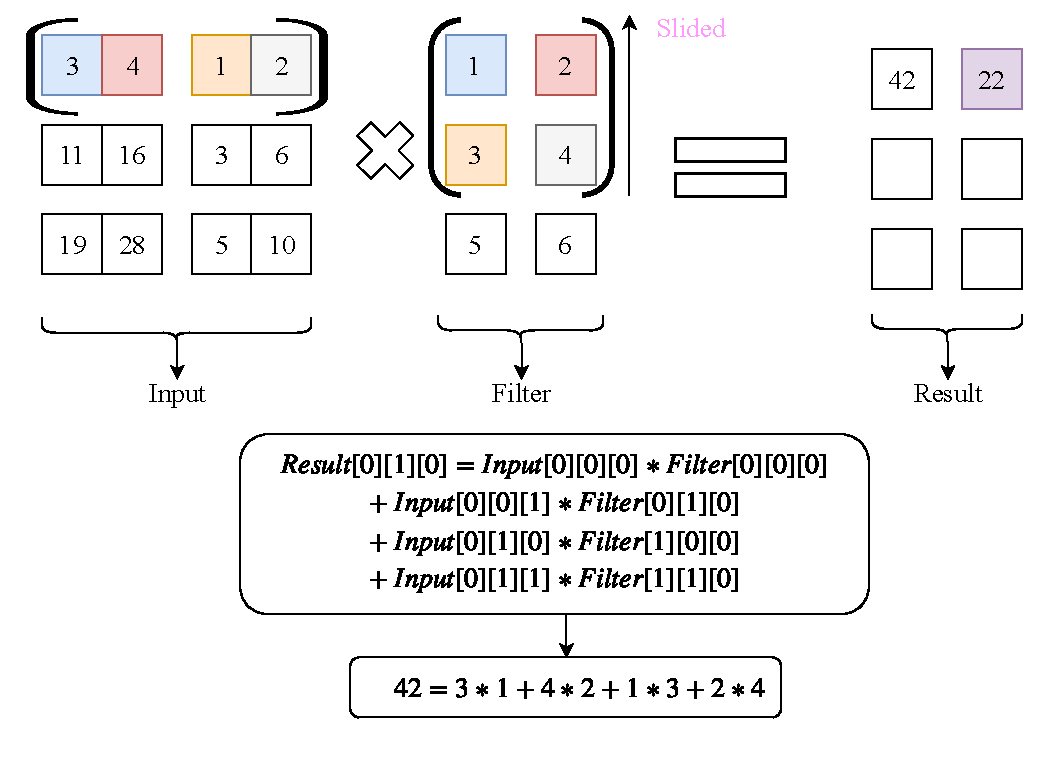
\includegraphics[width=\textwidth]{secondConvSample_step2}
	\end{center}
\end{blockfigure}
\newpage
\begin{blockfigure}{The entire convolution performed on the batch data.}
	\begin{center}
		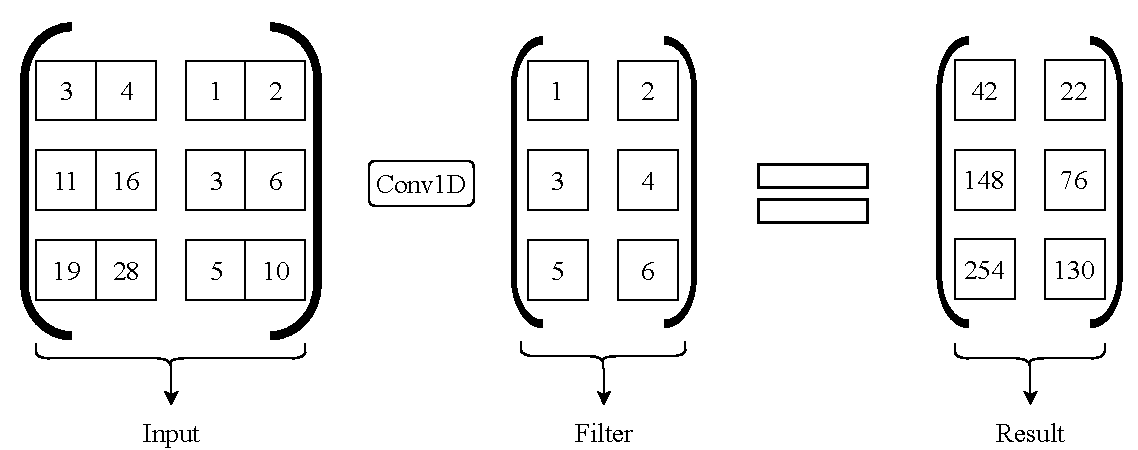
\includegraphics[width=\textwidth]{secondConvSample_final}
	\end{center}
\end{blockfigure}
\begin{blockfigure}{squeezing of the z-axis onto the y-axis.}
	\begin{center}
		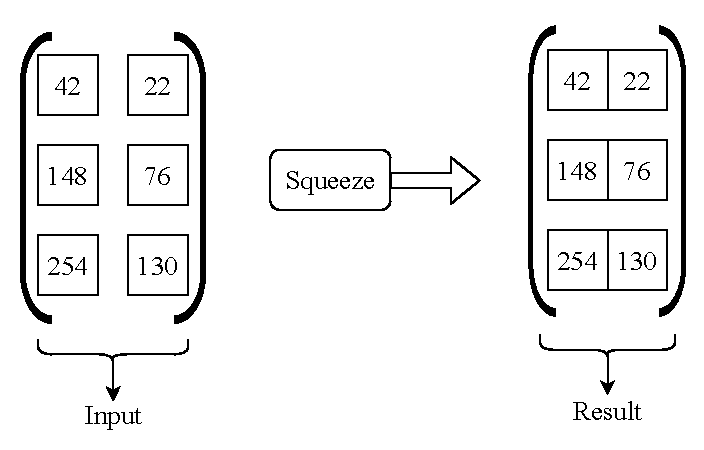
\includegraphics[width=\textwidth]{squeeze}
	\end{center}
\end{blockfigure}
\newpage
\begin{blockfigure}{ Net Graph Diagram - Alice}
	\begin{center}
		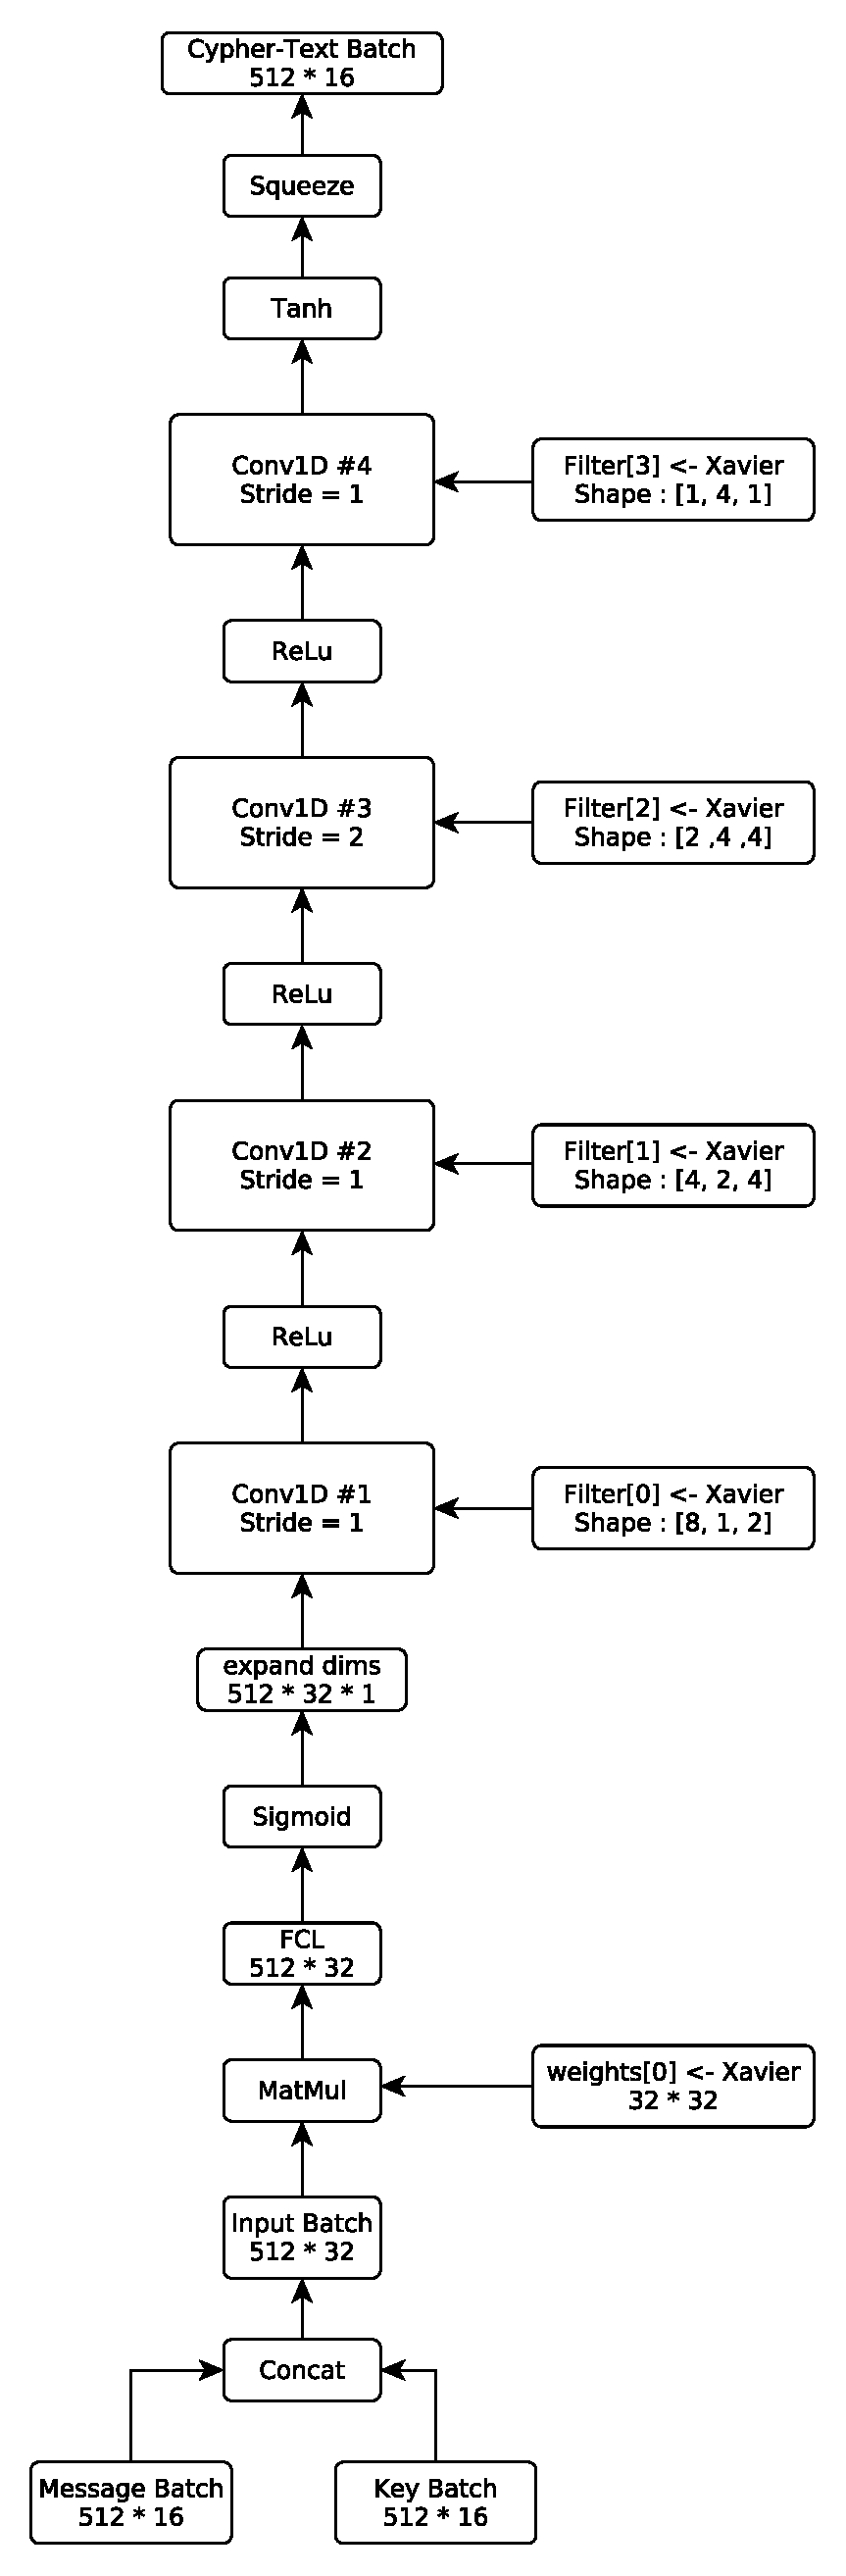
\includegraphics[height=0.93\textheight]{Alice-Diagram}
	\end{center}
\end{blockfigure}
\newpage
\begin{blockfigure}{ Net Graph Diagram - Bob}
	\begin{center}
		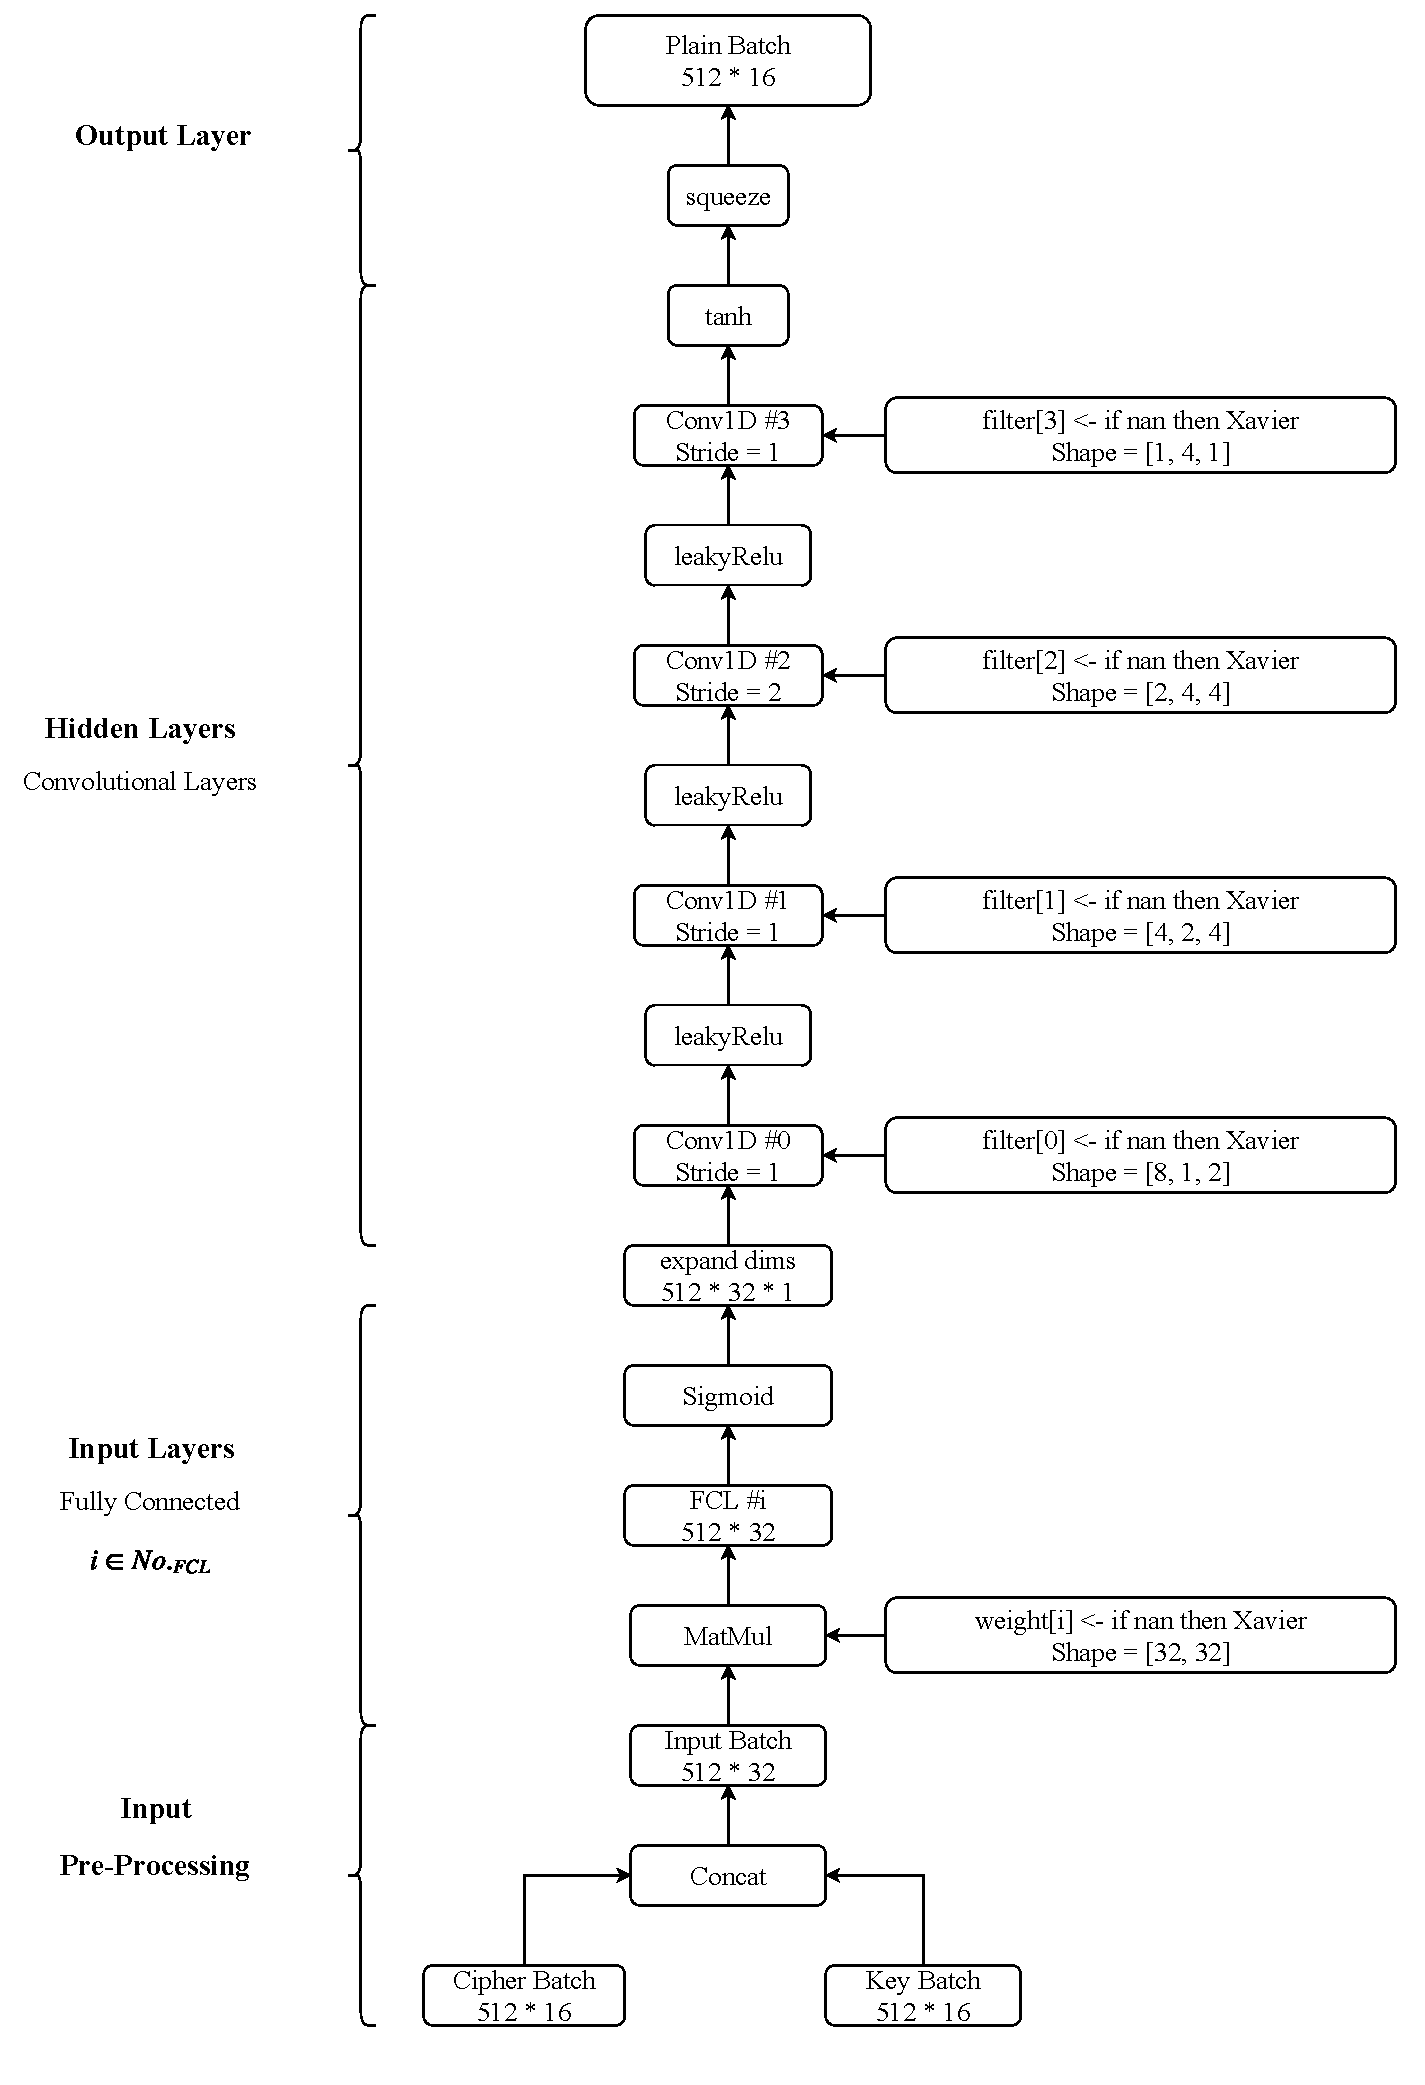
\includegraphics[height=0.93\textheight]{Bob-Diagram}
	\end{center}
\end{blockfigure}
\newpage
\begin{blockfigure}{ Net Graph Diagram - Eve/Alan}
		\begin{center}
			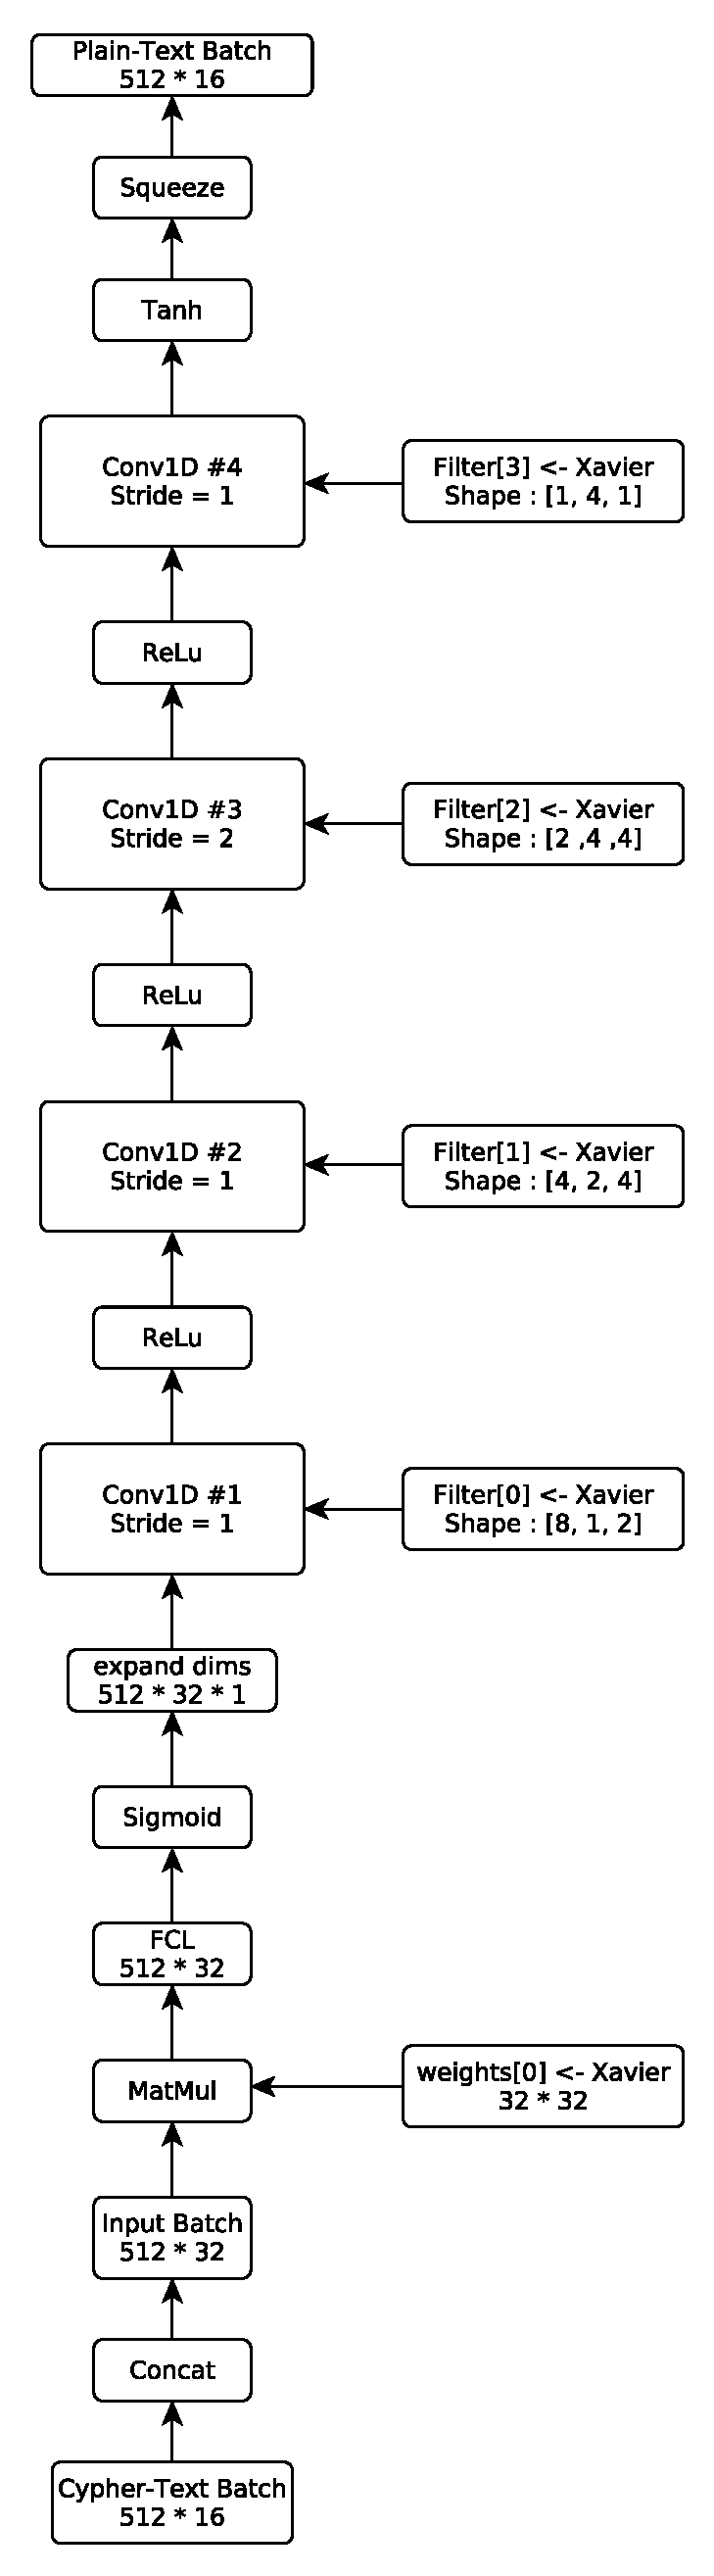
\includegraphics[height=0.93\textheight]{Eve-Diagram}
		\end{center}
\end{blockfigure}

\newpage
\section{\textbf{Design}}\label{sec:design}
\newpage
\section{\textbf{Implementation}}\label{sec:implementation}
\newpage
\section{\textbf{Conclusion}}\label{sec:conclusion}
\newpage

\medskip
\bibliographystyle{unsrt}
\bibliography{neurencoder}
\newpage

\appendix
\section*{\textbf{Appendix}}

\end{document}